% -*- TeX -*-
\documentclass{beamer}

\usepackage{amsmath}
\usepackage{array}
\usepackage{tikz}

\usetikzlibrary{decorations.pathreplacing}
\usetikzlibrary{fit,matrix}

\title{PyLith Modeling Tutorial}
\subtitle{Static Green's Functions}
\author{Charles Williams \\
  Brad Aagaard \\
  Matthew Knepley}
\institute{
\includegraphics[scale=0.4]{../../logos/cig_blackfg}}
\date{June 27, 2017}


% ---------------------------------------------------- CUSTOMIZATION
\renewcommand{\thispdfpagelabel}[1]{}
\newcommand{\pylith}[1]{{\color{green}#1}}
\newcommand{\python}[1]{{\color{red}#1}}
\usetheme{CIG}

\newcommand{\tensor}[1]{\overline{#1}}

% ========================================================= DOCUMENT
\begin{document}

% ------------------------------------------------------------ SLIDE
\maketitle

% ------------------------------------------------------------ SLIDE
\logo{
\includegraphics[height=4.5ex]{../../logos/cig_blackfg}}

% ========================================================== SECTION
\section{Static Greens' Functions}


% ========================================================== SUBSECTION
\subsection{Concepts covered}
% ------------------------------------------------------------ SLIDE
\begin{frame}
  \frametitle{Concepts Covered in this Session}
  \summary{}

  \begin{itemize}
  \item Simulation of a slow slip event (SSE) in Cascadia
  \item Usage of \pylith{SimpleGridDB} to specify fault slip
  \item Usage of a temporal database to specify variation of slip
    amplitude with time
  \item Solution output at a specified set of points
    (\pylith{OutputSolnPoints})
  \item Postprocessing of HDF5 output using \python{h5py}
  \item Generation of synthetic data with user-specified noise
  \item Generation of Green's functions in 3D
  \item Simple linear inversion using \python{numpy}
  \item Plotting of inversion results using \python{matplotlib} and
    \python{h5py}
  \end{itemize}
  
\end{frame}


% ========================================================== SUBSECTION
\subsection{Overview}

% ------------------------------------------------------------ SLIDE
\begin{frame}
  \frametitle{Green's Functions}
  \summary{}

  \begin{itemize}
  \item Compute deformation due to unit (i.e., 1 m) slip at fault
    vertices for use in an inversion for fault slip
    \begin{itemize}
    \item Slip decreases {\bf linearly} to 0 at surrounding vertices
    \item Similar but not equivalent to uniform slip over a patch
      (Okada dislocation)
    \item PyLith interpolates the responses to user-specified points
      using \pylith{OutputSolnPoints} output manager
    \end{itemize}
  \item Provides ability to compute Green's functions with arbitrarily
    complex elastic structure and/or topography
  \end{itemize}
  
\end{frame}


% ========================================================== SUBSECTION
\subsection{Other examples}
% ------------------------------------------------------------ SLIDE
\begin{frame}
  \frametitle{Other Green's Functions Examples}
  \summary{}

  \begin{itemize}
  \item 2-D examples: {\tt\color{red} examples/2d/greensfns}
    \begin{itemize}
    \item Example components
      \begin{enumerate}
      \item Compute synthetic (fake) observations for an earthquake
      \item Compute displacements at sites for Green's functions
      \item Invert for fault slip
      \end{enumerate}
    \item See Section 7.15 of the PyLith User Manual
    \end{itemize}
  \item 3-D example: {\tt\color{red} examples/3d/hex8/step21}
    \begin{itemize}
    \item Limited to computing displacements at sites for Green's functions
    \item No inversion
    \end{itemize}
  \end{itemize}
  
\end{frame}


% ========================================================== SECTION
\subsection{Cascadia example}

% ------------------------------------------------------------ SLIDE
\begin{frame}
  \frametitle{Cascadia Green's Functions Example}
  \summary{Simulated slow slip event plus inversion}

  \vfill
  Files are in {\tt\color{red} examples/3d/subduction}
  \vfill

  \begin{enumerate}
  \item Create a slip distribution that has a Gaussian shape spatially
    with a temporal variation, usting the Python script
    \python{subduction/spatialdb/generate\_slowslip.py}
  \item Run example {\tt step06.cfg} to generate a synthetic slow slip
    event
  \item Create synthetic observations with noise by running the Python
    script \python{subduction/make\_synthetic\_gpsdisp.py}
  \item Compute displacements at sites for Green's functions by
    running {\tt step07a.cfg} and {\tt step07b.cfg}
  \item Invert for fault slip using Python script
    \python{subduction/slip\_invert.py}
  \item Visualize inversion results using matplotlib Python package
    \python{subduction/viz/plot\_inversion\_misfit.py} and ParaView
  \end{enumerate}
  
\end{frame}


% ========================================================== SECTION
\subsection{Forward model}

% ------------------------------------------------------------ SLIDE
\begin{frame}
  \frametitle{Simulated Cascadia SSE}
  \summary{Time-varying slip on subduction interface}

  \vfill
  \begin{center}
    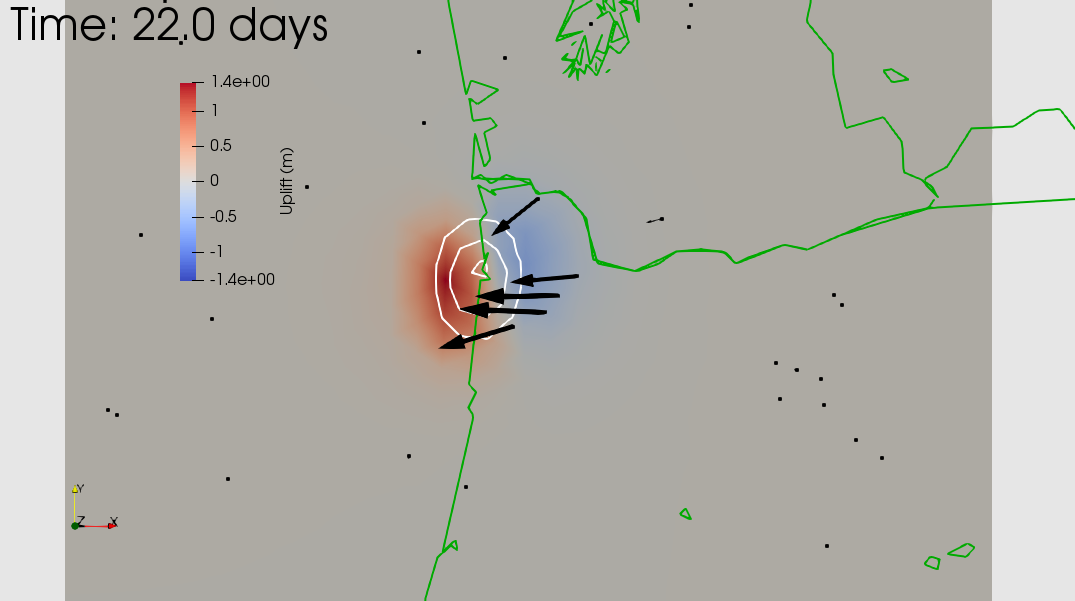
\includegraphics[height=6.1cm]{figs/subduction3d_step06_soln}
  \end{center}
  \vfill
  
\end{frame}


% ========================================================== SECTION
\subsection{Linear inversion}

% ------------------------------------------------------------ SLIDE
\begin{frame}
  \frametitle{Simple Linear Inversion}
  \summary{Parameters}

  \begin{description}
  \item[\textit{G}] Green's function matrix
  \item[\textit{d}] Unknown fault slip
  \item[\begin{math}d_{apriori}\end{math}] A priori estimate of fault slip
  \item[\begin{math}u_{obs}\end{math}] Observed displacement
  \item[\textit{D}] Penalty matrix
  \item[\begin{math}\theta\end{math}] Penalty parameter
  \end{description}
  
  \vfill The matrix \begin{math}{G_{ij}}\end{math} gives displacement
  component \textit{i} due to a unit of slip from component \textit{j}.
\vfill

\end{frame}


% ------------------------------------------------------------ SLIDE
\begin{frame}
  \frametitle{Simple Linear Inversion}
  \summary{Equations}

  \begin{itemize}
  \item Original system of equations:
    \begin{equation}
      G d = u_{obs}
    \end{equation}

  \item Augmented system of equations:
    \begin{equation}
      G_a d = u_a \text{, where } 
      G_a = \left[ \begin{array}{c} G \\ \theta D \end{array} \right]
      \text{ and }
      u_a = \left[ \begin{array}{c} u_{obs} \\ d_{apriori} \end{array} \right]
    \end{equation}
    
  \item Generalized inverse:
    \begin{gather}
      G^{-g} = \left( G_a^T G_a \right)^{-1} G_a^T \\
      d_{est} = G^{-g} u_a
    \end{gather}
  \end{itemize}
  
\end{frame}


% ========================================================== SECTION
\subsection{Inversion results}

% ------------------------------------------------------------ SLIDE
\begin{frame}
  \frametitle{Inversion results}
  \summary{Plot of weighted data misfit vs. penalty misfit}

  \vfill
  \begin{center}
    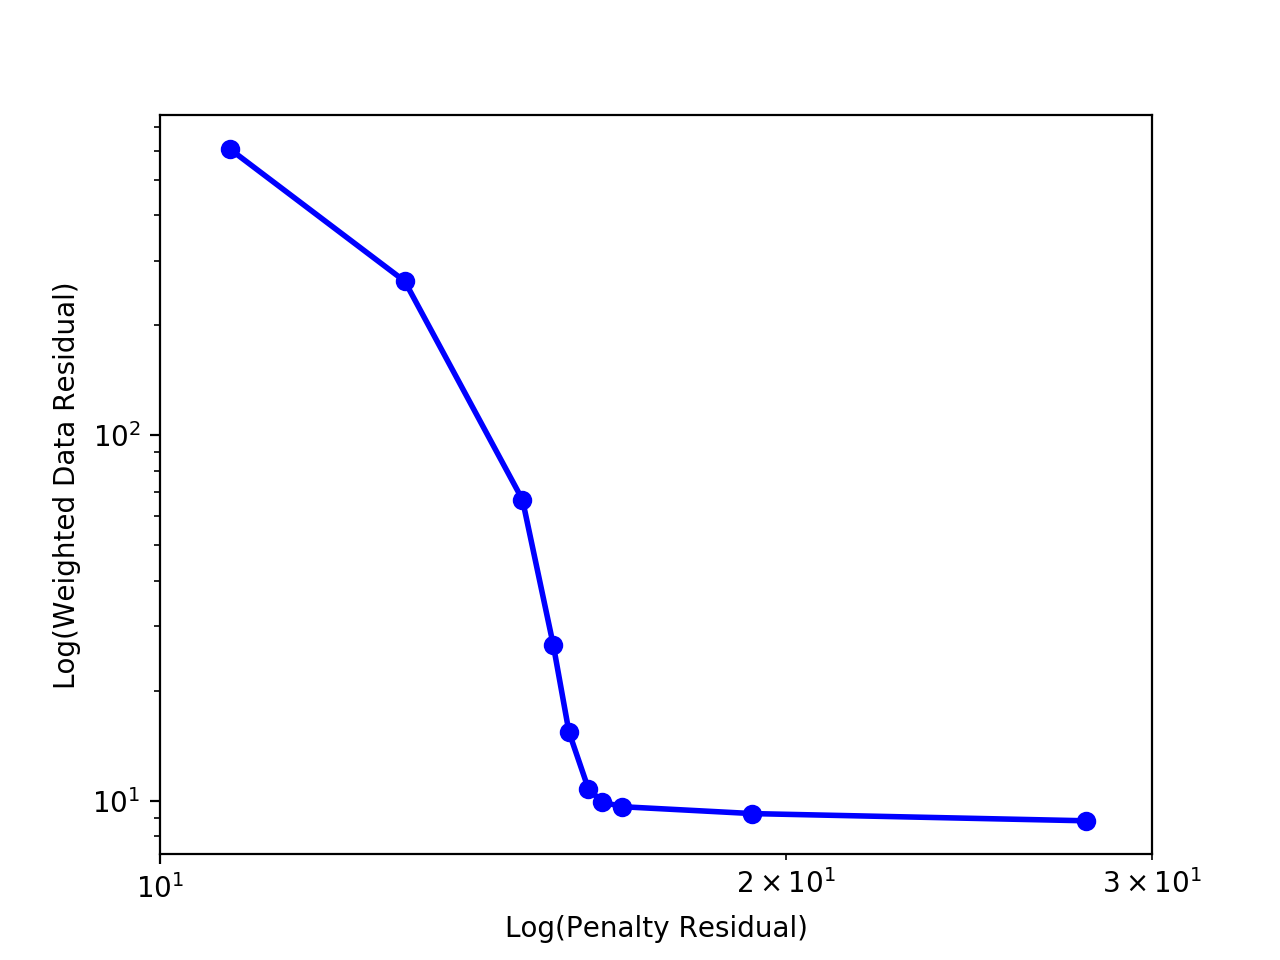
\includegraphics[height=6.1cm]{figs/subduction3d_step07_inverse_curve}
  \end{center}
  \vfill
  
\end{frame}


% ------------------------------------------------------------ SLIDE
\begin{frame}
  \frametitle{Inversion results}
  \summary{Predicted slip distribution}

  \vfill
  \begin{center}
    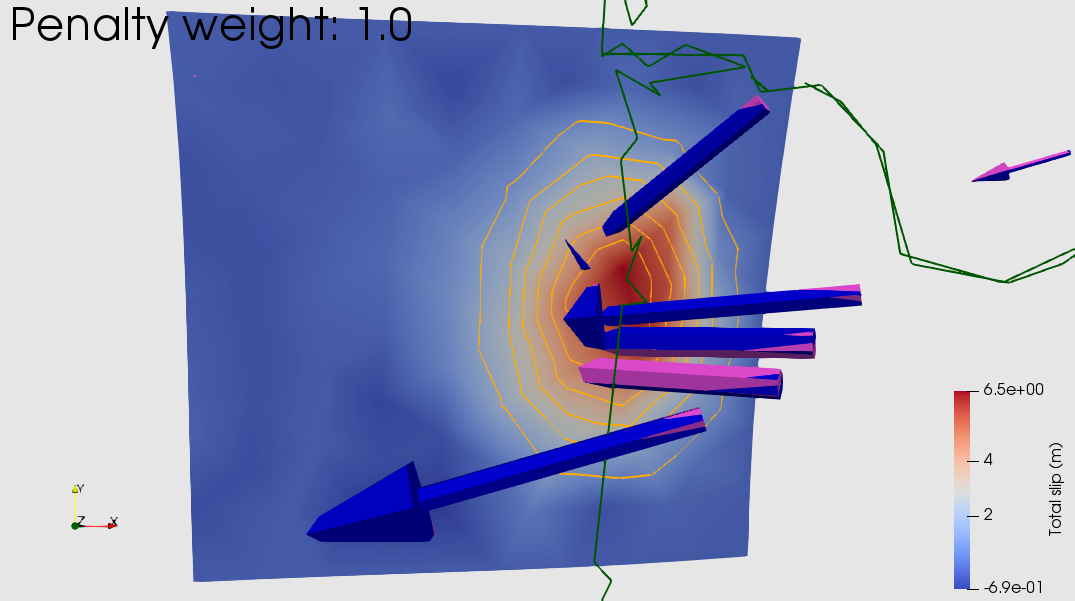
\includegraphics[height=6.1cm]{figs/subduction3d_step07_inverse_soln}
  \end{center}
  \vfill
  
\end{frame}

% ======================================================================
\end{document}


% End of file
